\section{Round Robin}

Con esta nueva estrategia, podemos enfrentar el problema que tiene FCFS con las tareas de corta duraci\'on. SchedRR es el primer algoritmo que presentamos en el trabajo que usa desalojo. Cada vez que se produce un click de reloj, el algoritmo decide cu\'al es la tarea a la que se le asigna el procesador.

En la primera de las estrategias \textit{round robin}, de acuerdo a lo solicitado en el \textbf{ejercicio 3}, se usa una \'unica cola global. Cuando una tarea est\'a lista para ejecutarse pasa a esta cola, a la que llamaremos cola de ready. 

Peri\'odicamente, cuando se produce la interrupci\'on de reloj, se verifica si finaliz\'o el quantum del n\'ucleo correspondiente. Si es as\'i, la estrategia toma el primer elemento de la cola, lo saca de ella y le asigna el procesador. En caso de que la cola se encuentre vac\'ia, se ejecuta la tarea IDLE. La tarea que se encontraba ejecutando, si todav\'ia no termin\'o, se vuelve a encolar.

Cuando una tarea se bloquea por pedido de E/S, sale de la cola de READY. Reci\'en vuelve a encolarse cuando se desbloquea.

Esta estrategia se encuentra implementada en los archivos \verb+sched_rr.h+ y \verb+sched_rr.cpp+. La cola se define en el header como un atributo privado:

\begin{verbatim} 
std::queue<int> q;
\end{verbatim}

Tenemos atributos que nos sirven para manejar los quantums correspondientes a cada n\'ucleo:

\begin{verbatim}
        std::vector<int> contadorQuantums; // se usa para controlar los quantums
       std::vector<int> contadorQuantumsOriginal; // guardo la cantidad de 
               // quantums de cada nucleo
\end{verbatim}

contadorQuantums lo utilizaremos para saber en cada tick de reloj si se termin\'o el quantum, mientras que contadorQuantumsOriginal es un vector que guarda para cada n\'ucleo la cantidad de ticks (interrupciones de reloj) que abarca el quantum. 

El comportamiento frente al tick de reloj se define en la funci\'on \textit{tick}.

En caso de que el proceso desalojado termine, se toma el pr\'oximo en la cola. Si la cola est\'a vac\'ia, se retorna la \verb+TASK_IDLE+:

Esta funci\'on se ocupa tambi\'en de volver el contador del quantum del n\'ucleo correspondiente al valor original en caso de que el proceso salga o se bloquee, mientras que si el proceso se encuentra todav\'ia ejecut\'andose se fija si se agot\'o el quantum.

\begin{verbatim}
    if (m == EXIT) {
        // Si el pid actual terminó, sigue el proximo encolado
        if (q.empty()) return IDLE_TASK; // si la cola esta vacia, se retorna IDLE_TAS
        else {
            int sig = q.front(); q.pop(); // sino se toma el primero y se desencola
            return sig;
         }
    } 
\end{verbatim}

En el caso de que el proceso desalojado se bloquee por E/S, se sigue el mismo comportamiento:

\begin{verbatim}
    if (m == BLOCK) {
         if (!q.empty()) { // en caso de bloqueo se usa la misma estrategia
            int sig = q.front(); q.pop();
            return sig;
         } else {
             return IDLE_TASK; // si el único proceso está bloquedo
                             // ejecuta IDLE_TASK
         }
    }
\end{verbatim}

Si la tarea no termin\'o, se realiza lo mismo pero se vuelve a encolar la tarea desalojada:

\begin{verbatim}
    if (m == TICK) {
        if (!q.empty()) { // si se produjo una interrupcion de reloj se hace lo mismo
                   // pero se vuelve a encolar la tarea
            int sig = q.front(); q.pop();
            int des = current_pid(cpu);
            if (des != IDLE_TASK) {
                q.push(des); // vuelvo a encolar el proceso desalojado
            }
            return sig;
         } else {
               return current_pid(cpu);
         }
   }
\end{verbatim}

De acuerdo a lo pedido en el \textbf{ejercicio 4}, presentamos varios lotes de tareas, observ\'ando como el comportamiento se corresponde a la estrategia \textit{round robin}:


\begin{verbatim}
TaskCPU 3
TaskCPU 3
TaskCPU 3
TaskCPU 3
TaskCPU 3
\end{verbatim}

\begin{figure}[H]
\caption{5 TaskCPU sin llamadas de E/S, 1 core}
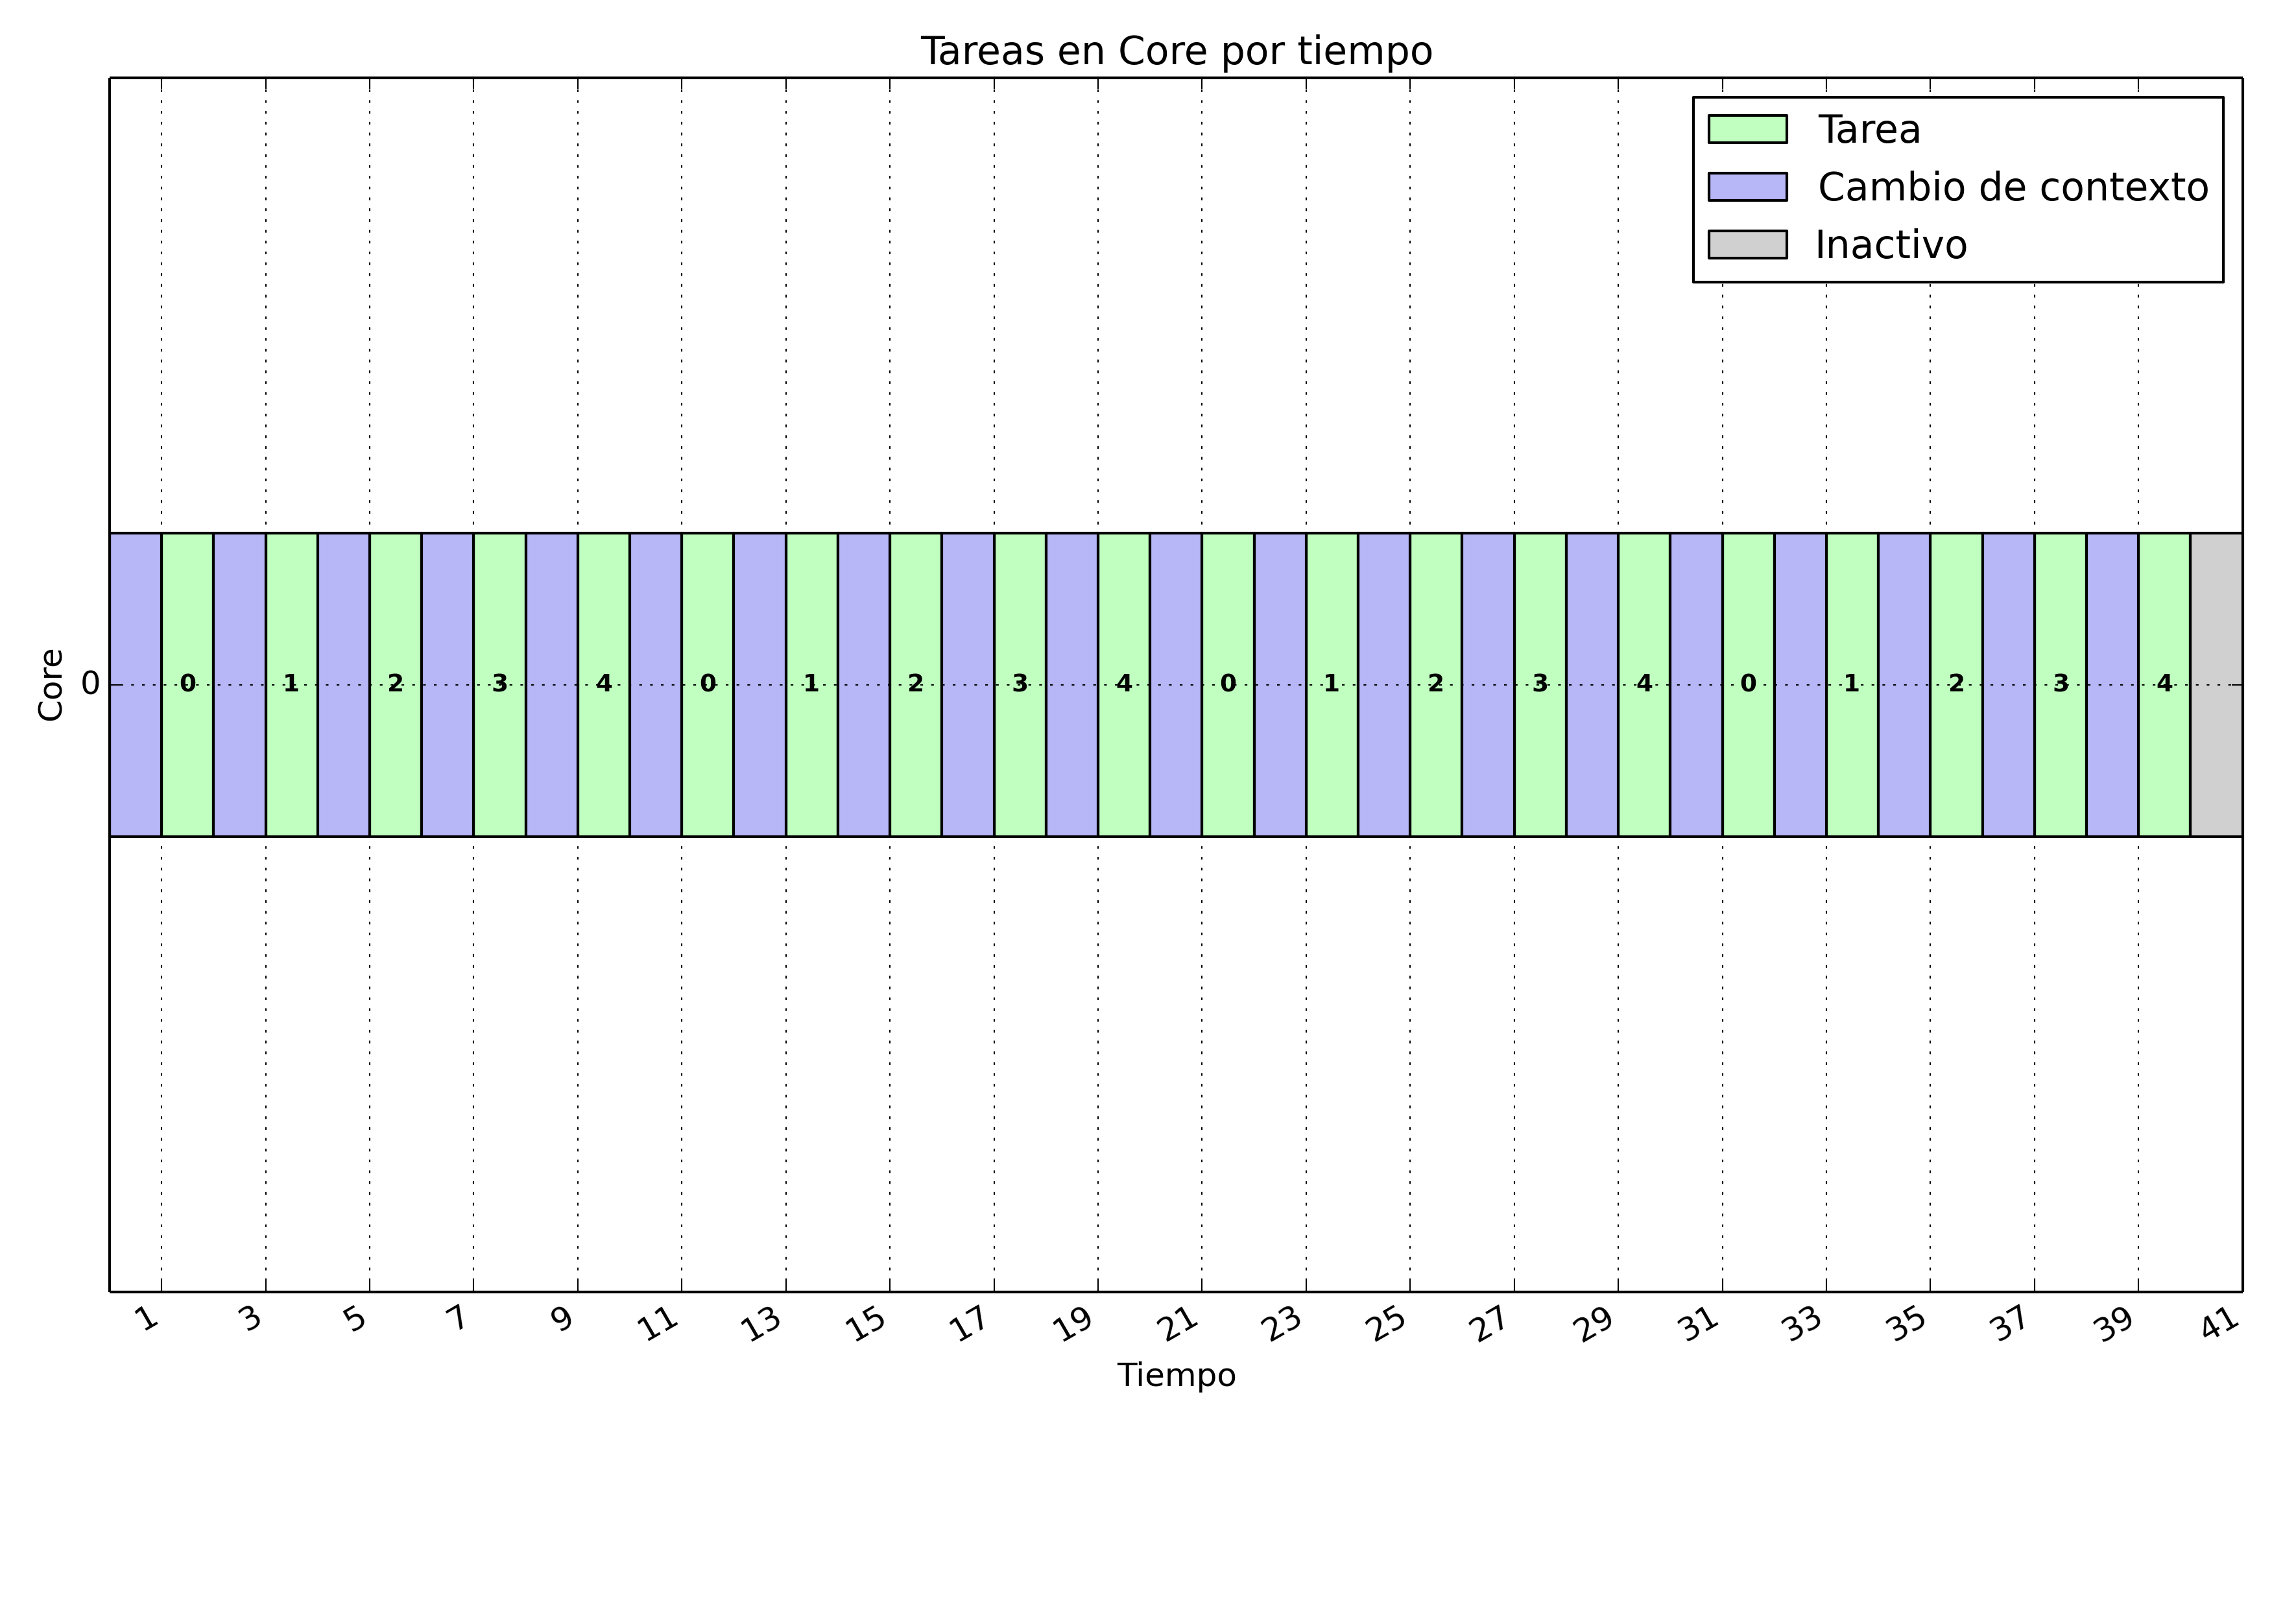
\includegraphics[width=\textwidth]{ejercicio_4_1}
\end{figure}

En este lote, se observa c\'omo act\'ua round-robin en un ambiente de un solo core. Las tareas se van alternando en el uso del procesador, con el tiempo necesario para el cambio de contexto. Cada vez que una tarea es desalojada, se vuelve a encolar hasta terminar su procesamiento. En este caso en particular, no se produjo ninguna llamada a E\S: cuando la tarea es desalojada vuelve en el mismo acto a la cola de READY. Vemos, entonces que la secuencia de ejecuci\'on fue: \verb+1-2-3-4-1-2-3-4...+

Ejecutamos el mismo lote pero con dos cores:

\begin{figure}[H]
\caption{5 TaskCPU sin llamadas de E/S, 2 cores}
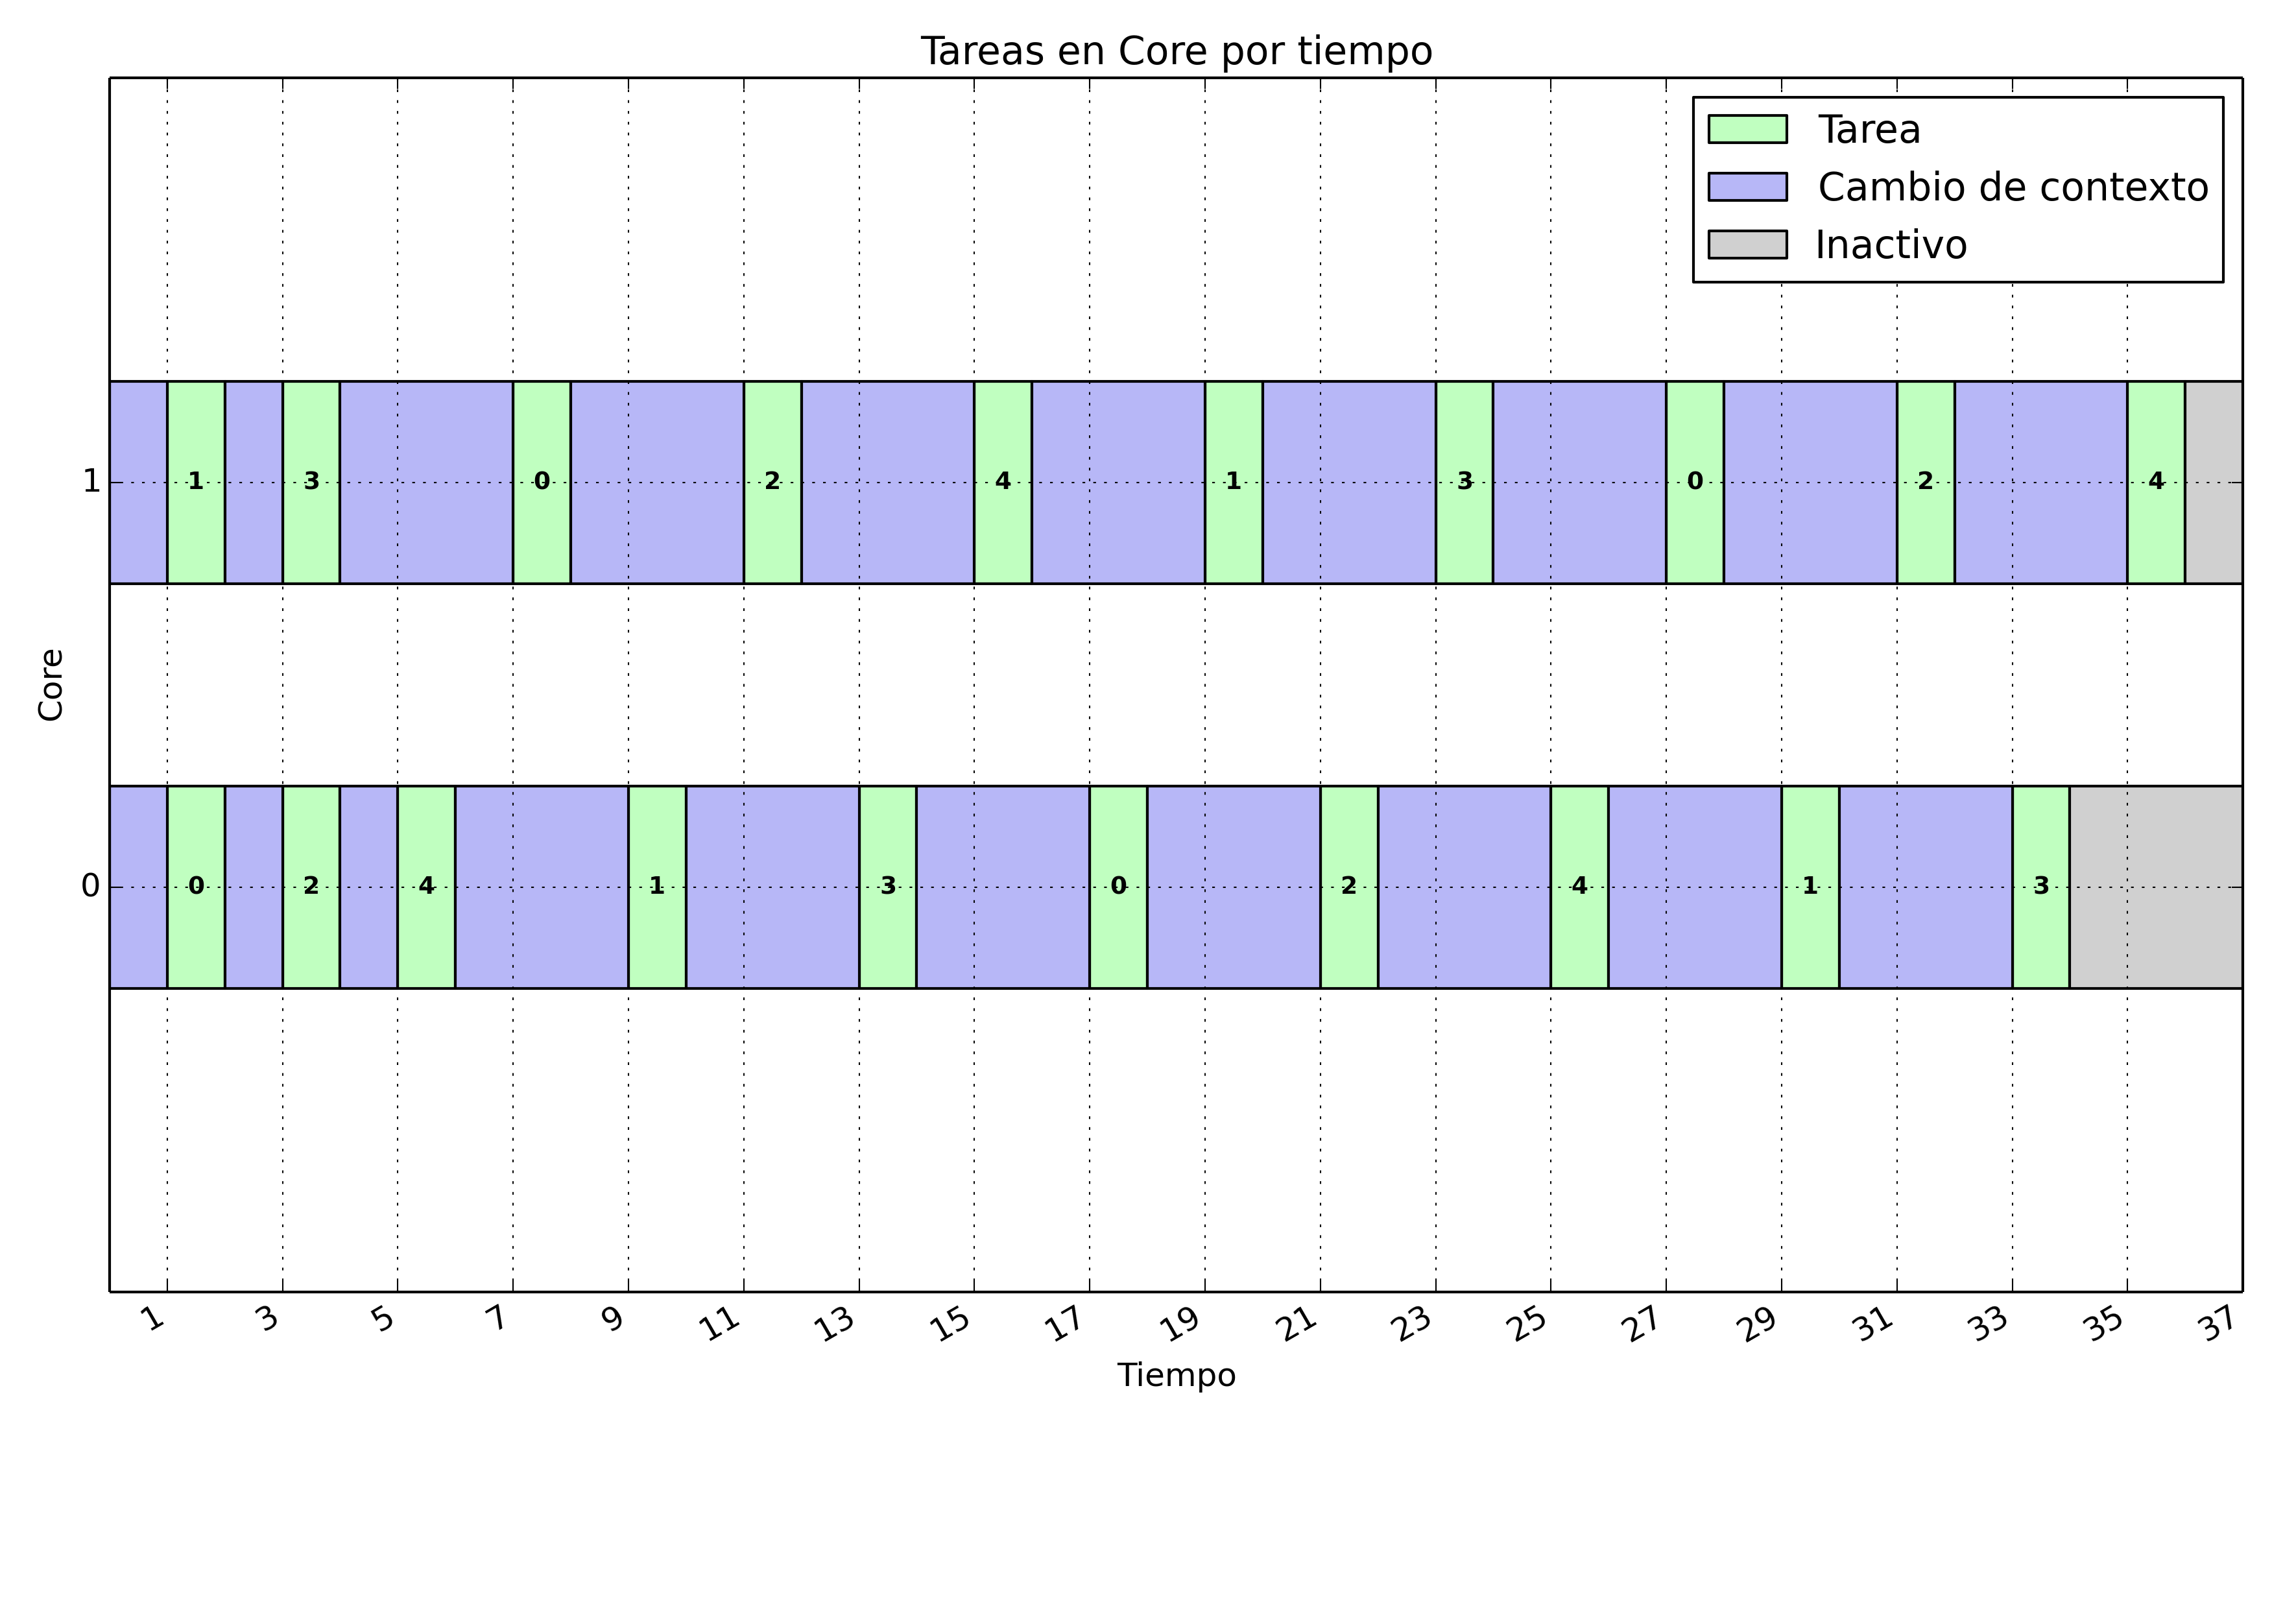
\includegraphics[width=\textwidth]{ejercicio_4_2}
\end{figure}

En este caso, vemos como al tener una \'unica cola global, se produce el pasaje de una tarea de un core a otro. 

Se debe notar que hasta al tick 4 de reloj, entre el quantum de cada tarea, nada m\'as tenemos el overhead del cambio de contexto. Sin embargo, al pasar las tareas a los otros cores, el overhead entre tarea aumenta ya que le pedimos que el cambio de core tome 2 ticks de reloj. Esta primera versi\'on de \textit{round robin} no toma en cuenta la penalidad de cambio de n\'ucleo, por lo que cuando se toma una tarea de la cola no se toma en cuenta si estuvo ejecutando en el otro core.

De todos modos, vemos como se contin\'ua globalmente la idea de una cola circular. La selecci\'on de la tarea asignada al core del tick sigue teniendo la secuencia \verb+1-2-3-4-1-2-3-4...+

Por \'ultimo, tomamos un lote con una tarea que llama a E/S y se bloquea:

\begin{verbatim}
TaskCPU 3
TaskConsola 3 5 10
TaskCPU 3
TaskCPU 3
TaskCPU 3
TaskCPU 3
\end{verbatim}

\begin{figure}[H]
\caption{5 TaskCPU y un TASKCONSOLE que llama a E/S, 1 core}
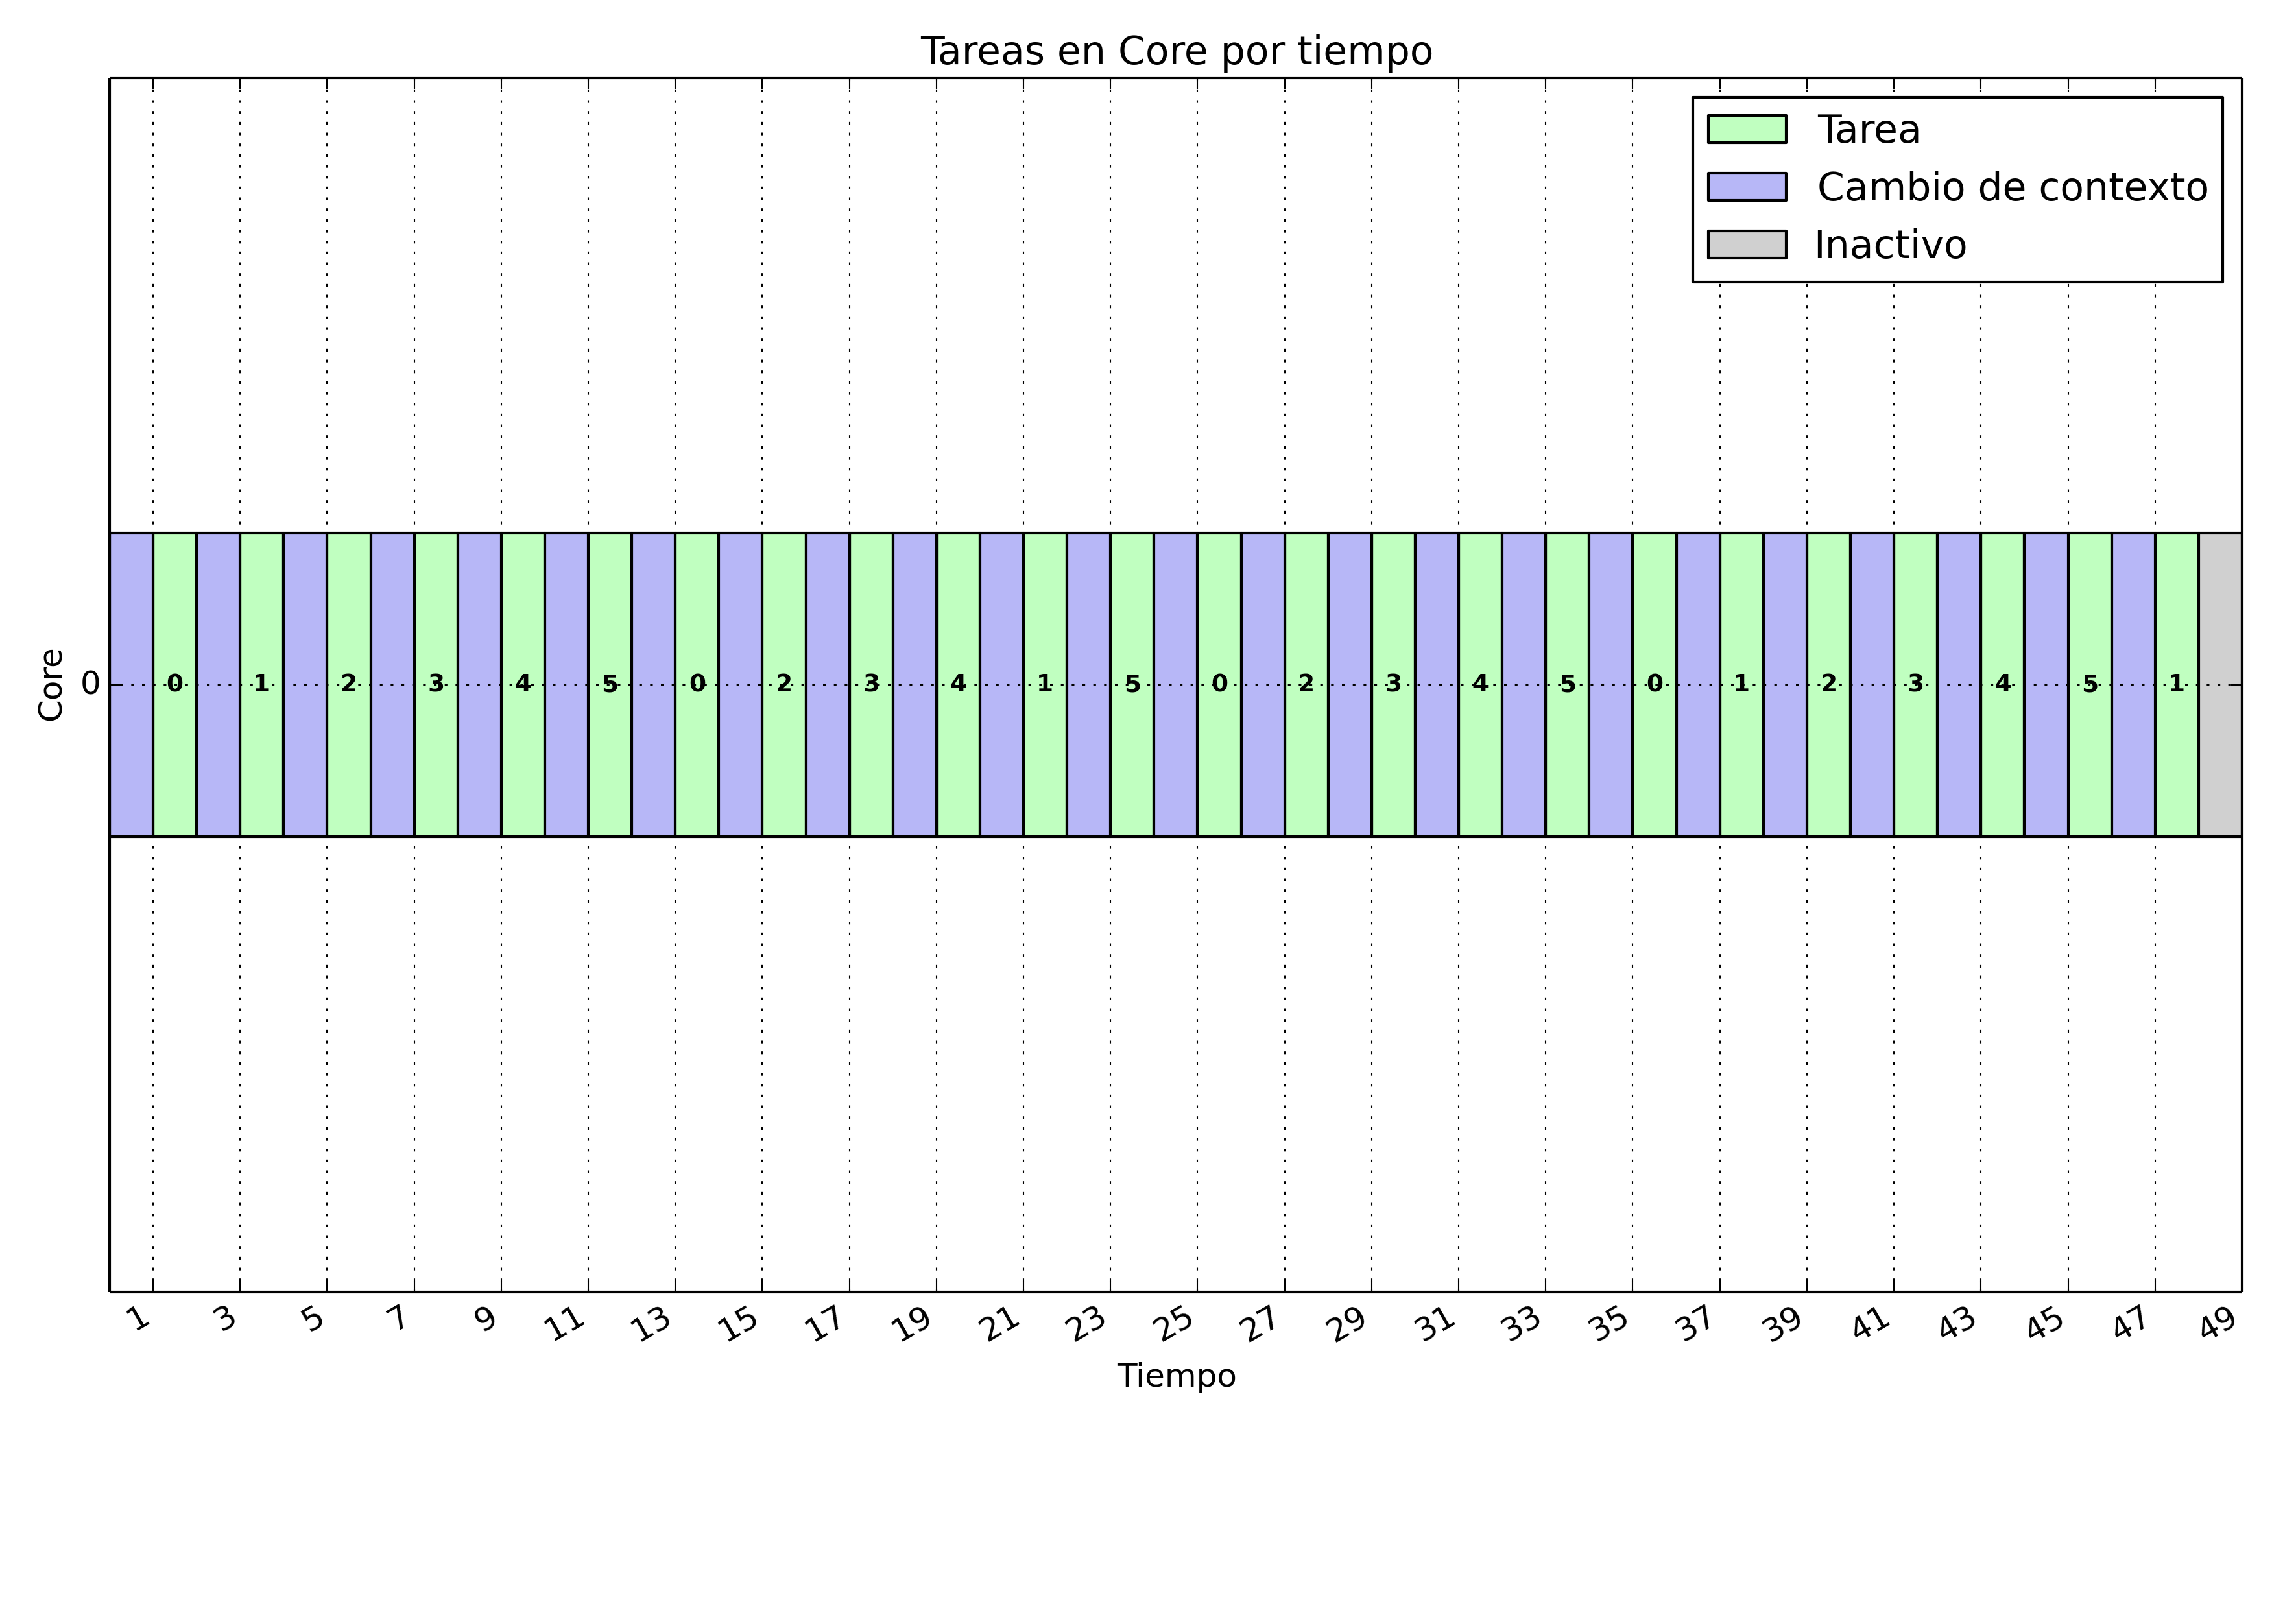
\includegraphics[width=\textwidth]{ejercicio_4_3}
\end{figure}

Observemos que en este caso la tarea 1 se bloquea y no veulve a la cola hasta tick 22.